	%Template by Mark Jervelund - D1 - 2015 - mjerv15@student.sdu.dk

\documentclass[a4paper,10pt,titlepage]{report}

\usepackage[utf8]{inputenc}
\usepackage[T1]{fontenc}
\usepackage[english]{babel}
\usepackage{amssymb}
\usepackage{amsmath}
\usepackage{amsthm}
\usepackage{graphicx}
\usepackage{fancyhdr}
\usepackage{lastpage}
\usepackage{listings}
\usepackage{algorithm}
\usepackage{algpseudocode}
\usepackage[document]{ragged2e}
\usepackage[margin=1in]{geometry}
\usepackage{color}
\usepackage{datenumber}
\usepackage{venndiagram}
\usepackage{chngcntr}
\setdatetoday
\addtocounter{datenumber}{0} %date for dilierry standard is today
\setdatebynumber{\thedatenumber}
\date{}
\setcounter{secnumdepth}{0}
\pagestyle{fancy}
\fancyhf{}

\newcommand{\Z}{\mathbb{Z}}
\lhead{Database Management Systems (DM556))}
\rhead{Mark Jervelund (Mjerv15) Troels B. Petersen (trpet15)}
\rfoot{Page  \thepage \, of \pageref{LastPage}}
\counterwithin*{equation}{section}

\lstset{
  numbers=left,
  stepnumber=5,
  firstnumber=1,
  numberfirstline=true
  frame=single,
  breaklines=true,
  postbreak=\raisebox{0ex}[0ex][0ex]{\ensuremath{\color{red}\hookrightarrow\space}}
}

\begin{document}
\begin{titlepage}
\centering
    \vspace*{9\baselineskip}
    \huge
    \bfseries
    Project 3\\

    \normalfont
	\huge
    Database Management Systems (DM556)  \\[4\baselineskip]
    \normalfont
	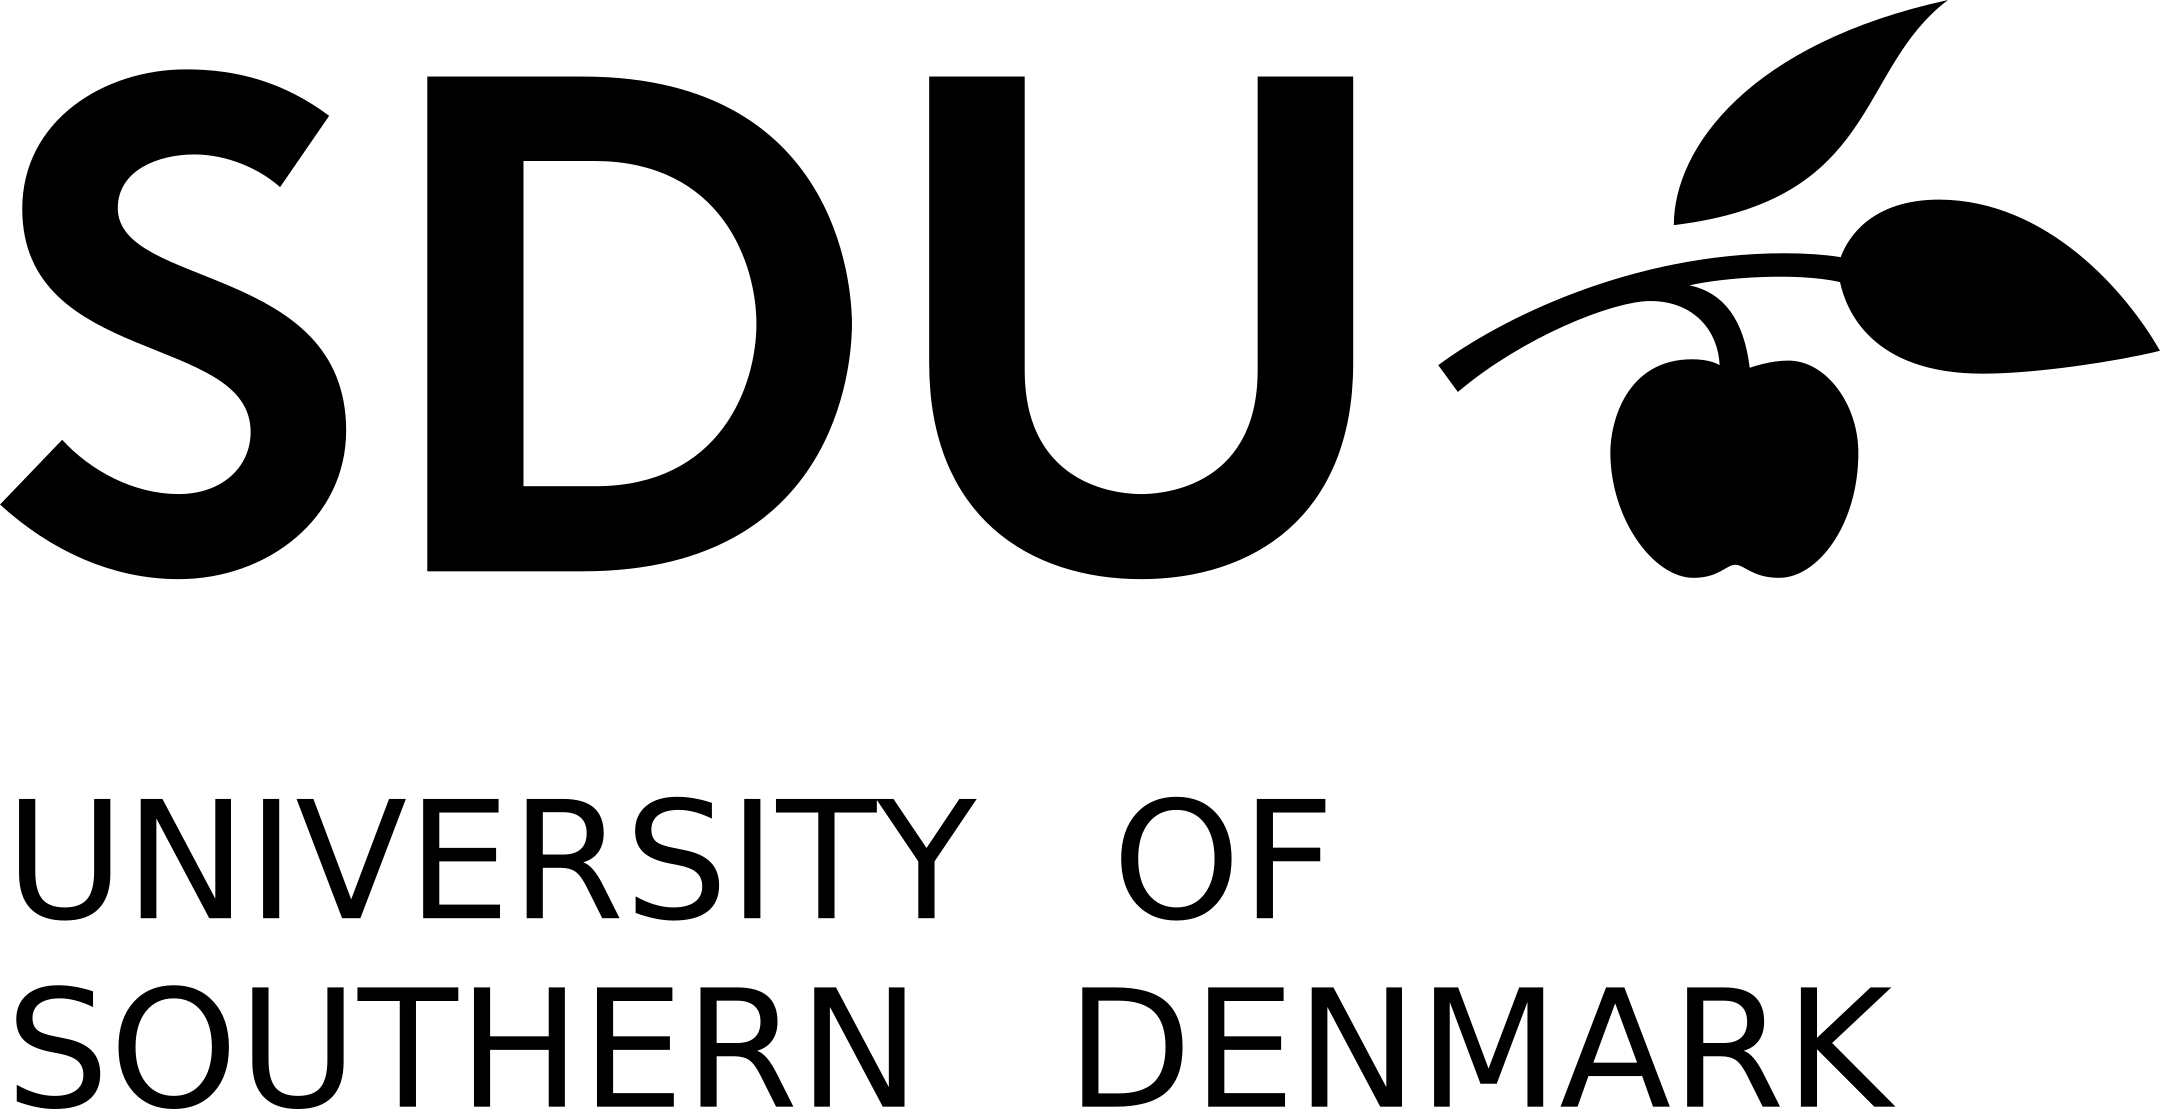
\includegraphics[scale=1.5]{SDU_Logo}
    \vfill\
    Group 2\\
    Mark Jervelund (Mjerv15)    Troels B. Petersen (trpet15)
    \vspace{5mm}
    IMADA \\
    \textbf{\datedate} \\[2\baselineskip]
\end{titlepage}
%\renewcommand{\thepage}{\roman{page}}% Roman numerals for page counter
%\tableofcontents

%\newpage
\setcounter{page}{1}
\renewcommand{\thepage}{\arabic{page}}

\lstset{language=Java}          % Set your language (you can change the language for each code-block optionally)

\section{Project 1}
BuffMgr.java and clock.java in bufmgr \\


\subsection{bufMgr.java} 

\subsubsection{public bufmgr(int numbufs)}
init function that initializes the bufpool and the frame tap. as well as building the pagemap and selecting the replacement function.
\subsubsection{public PageId newPage(Page firstpg, int run\_size)}
Loads a new page into the buffer pool, and calls the pinpage function on the first page, if sucssesful calls the replacer to put the page in the frametab, and returns the pageid id. or throws RuntimeException if it fails to pin the page.

\subsubsection{public void pinPage(PageId pageno, Page page, boolean skipRead)}
Pins a disk page into the buffer pool. If the page is already pinned,
this simply increments the pin count. Otherwise, this selects another
page in the pool to replace, flushing the replaced page to disk if
it is dirty.
\vspace{5mm}
\\
If one needs to copy the page from the memory instead of reading from
the disk, one should set skipRead to PIN\_MEMCPY. In this case, the page
shouldn't be in the buffer pool. \\ Throw an IllegalArgumentException if so. )

\subsubsection{  public void unpinPage(PageId pageno, boolean dirty) throws IllegalArgumentException }
Unpins a disk page from the buffer pool, decreasing its pin count. and marks it as dirty in the pagemap if the boolean dirty is true.
\vspace{5mm}

\subsubsection{public void flushPage(PageId pageno}
Flushes a single page to disk if dirty, else just does nothing.

\subsubsection{public void flushAllPages(}
Calls the flush page on all pages in the buffer to disk using the flush page function so only the dirty ones get written.

\subsubsection{public void getNumBuffers}
return the length of the buffer pool

\subsubsection{public int getNumUnpinned}

Loops over the frame tab and counts how many pages are pinned at any given time.

\vspace{5mm}
\subsection{clock.java} 
pickvictim \\
Gets the first page in the frametab with pincount 0. \\
This means that we remove the first page in the buffer that no one else is using, if there are no free pages then we return -1 and signalling the parent function that there is no free pages in the buffer pool at the moment.


\section{Project 2}

\subsection{projection.java} 

\subsection{selection.java} 

\subsection{mergejoin.java} 


\section{OProject 3}

\end{document}